\documentclass[landscape,a0paper,fontscale=0.292]{baposter}

\usepackage[vlined]{algorithm2e}
\usepackage{times}
\usepackage{calc}
\usepackage{url}
\usepackage{graphicx}
\usepackage{amsmath}
\usepackage{amssymb}
\usepackage{relsize}
\usepackage{multirow}
\usepackage{booktabs}
\usepackage{import}
\usepackage{graphicx}
\usepackage{multicol}
\usepackage{xcolor}
\usepackage[T1]{fontenc}
\usepackage{ae}

\graphicspath{{images/}}

\definecolor{uoh}{HTML}{04a0ff}
\definecolor{textouoh}{HTML}{FFFAFF}
\definecolor{textouohobscuro}{HTML}{42515b}


%%%%%%%%%%%%%%%%%%%%%%%%%%%%%%%%%%%%%%%%%%%%%%%%%%%%%%%%%%%%%%%%%%%%%%%%%%%%%
%% Begin of Document
%%%%%%%%%%%%%%%%%%%%%%%%%%%%%%%%%%%%%%%%%%%%%%%%%%%%%%%%%%%%%%%%%%%%%%%%%%%%%
\begin{document}
%%%%%%%%%%%%%%%%%%%%%%%%%%%%%%%%%%%%%%%%%%%%%%%%%%%%%%%%%%%%%%%%%%%%%%%%%%%%%
%% Here starts the poster
%%---------------------------------------------------------------------------
%% Format it to your taste with the options
%%%%%%%%%%%%%%%%%%%%%%%%%%%%%%%%%%%%%%%%%%%%%%%%%%%%%%%%%%%%%%%%%%%%%%%%%%%%%
\begin{poster}{
 % Show grid to help with alignment
 grid=false,
 % Column spacing
 colspacing=0.7em,
 % Color style
 headerColorOne=uoh,
 borderColor=uoh,
 % Format of textbox
 %textborder=faded,
 % Format of text header
 headerborder=open,
 headershape=roundedright,
 headershade=plain,
 background=none,
 bgColorOne=cyan!10!white,
 headerheight=0.12\textheight}
 % Eye Catcher
 {
      
\includegraphics[width=0.08\linewidth]{qr}
 }
 % Title
 {\LARGE {\input{/Users/hectorbahamonde/RU/Dissertation/Papers/Earthquake_Paper/title.txt}\unskip}}
 % Authors
 {{\bf{\color{uoh}Hector Bahamonde, PhD}}\\[1em]
 {\texttt{Hector.Bahamonde@uoh.cl \hspace{1cm} www.HectorBahamonde.com \hspace{1cm} Instituto de Ciencias Sociales}}}
 % University logo
 {
  %\begin{tabular}{r}
    
\includegraphics[height=0.25\textheight]{logo}
  %\end{tabular}
 }

%%%%%%%%%%%%%%%%%%%%%%%%%%%%%%%%%%%%%%%%%%%%%%%%%%%%%%%%%%%%%%%%%%%%%%%%%%%%%%
%%% Now define the boxes that make up the poster
%%%---------------------------------------------------------------------------
%%% Each box has a name and can be placed absolutely or relatively.
%%% The only inconvenience is that you can only specify a relative position 
%%% towards an already declared box. So if you have a box attached to the 
%%% bottom, one to the top and a third one which should be inbetween, you 
%%% have to specify the top and bottom boxes before you specify the middle 
%%% box.
%%%%%%%%%%%%%%%%%%%%%%%%%%%%%%%%%%%%%%%%%%%%%%%%%%%%%%%%%%%%%%%%%%%%%%%%%%%%%%

%%%%%%%%%%%%%%%%%%%%%%%%%%%%%%%%%%%%%%%%%%%%%%%%%%%%%%%%%%%%%%%%%%%%%%%%%%%%%%
  \headerbox{{\color{textouoh}Contribution and Main Findings}}{name=sectionA,column=0,row=0,span=2}{
%%%%%%%%%%%%%%%%%%%%%%%%%%%%%%%%%%%%%%%%%%%%%%%%%%%%%%%%%%%%%%%%%%%%%%%%%%%%%%
Income taxation fostered via spillover effects increases in state-consolidation over time in Chile. I created a novel hand-collected longitudinal dataset on Chilean earthquake death tolls (N=103). Death tolls decrease (state capacity increases) once the income tax law was implemented in 1924. A sector approach is leveraged.
}
%%%%%%%%%%%%%%%%%%%%%%%%%%%%%%%%%%%%%%%%%%%%%%%%%%%%%%%%%%%%%%%%%%%%%%%%%%%%%%
\headerbox{{\color{textouoh}Gaps in the Literature}}{name=sectionB,column=0,below=sectionA}{
%%%%%%%%%%%%%%%%%%%%%%%%%%%%%%%%%%%%%%%%%%%%%%%%%%%%%%%%%%%%%%%%%%%%%%%%%%%%%%
\begin{enumerate}
	\item The Literature has overlooked fiscal development in the developing countries.
		\begin{itemize}
			\item Most theories explain European cases.
			\item Focus is on external conflicts (wars): taxation and war.
			\item Latin America has not seen the degree of conflict Europe had.
		\end{itemize}
	\item A measurement to capture overtime levels of state-capacity is lacking.
		\begin{itemize}
			\item Most measurements capture contemporaneous levels of state-capacity: experimental and observational work.
			\item However, we know that factors such as colonial legacies played an important role fostering/limiting state-capacity.
		\end{itemize}
\end{enumerate}

}



 %%%%%%%%%%%%%%%%%%%%%%%%%%%%%%%%%%%%%%%%%%%%%%%%%%%%%%%%%%%%%%%%%%%%%%%%%%%%%%
\headerbox{{\color{textouoh}Earthquake Data: Geographical Distribution}}{name=sectionC,column=2,row=0,span=2}{
 %%%%%%%%%%%%%%%%%%%%%%%%%%%%%%%%%%%%%%%%%%%%%%%%%%%%%%%%%%%%%%%%%%%%%%%%%%%%%%
  

\begin{minipage}{.4\linewidth}
	\begin{itemize}
		\item Exploiting the {\bf exogeneity} of {\bf earthquake shocks}, I leveraged a novel hand-collected dataset on Chilean earthquake death tolls between 1900 and 2010.
		\item Earthquakes are {\bf time-invariant}, and importantly, orthogonal to economic development and regime type.
		\item[{\LARGE{\bf{\color{red}$\star$}}}] Under reasonable assumptions, if the state's capacity for enforcing and monitoring building codes throughout the territory is a reflection of overall state capacity, then death-toll differentials should be mainly associated with state capacity.
	\end{itemize}
	 
\end{minipage}
  \begin{minipage}{.7\linewidth}
    \centering
    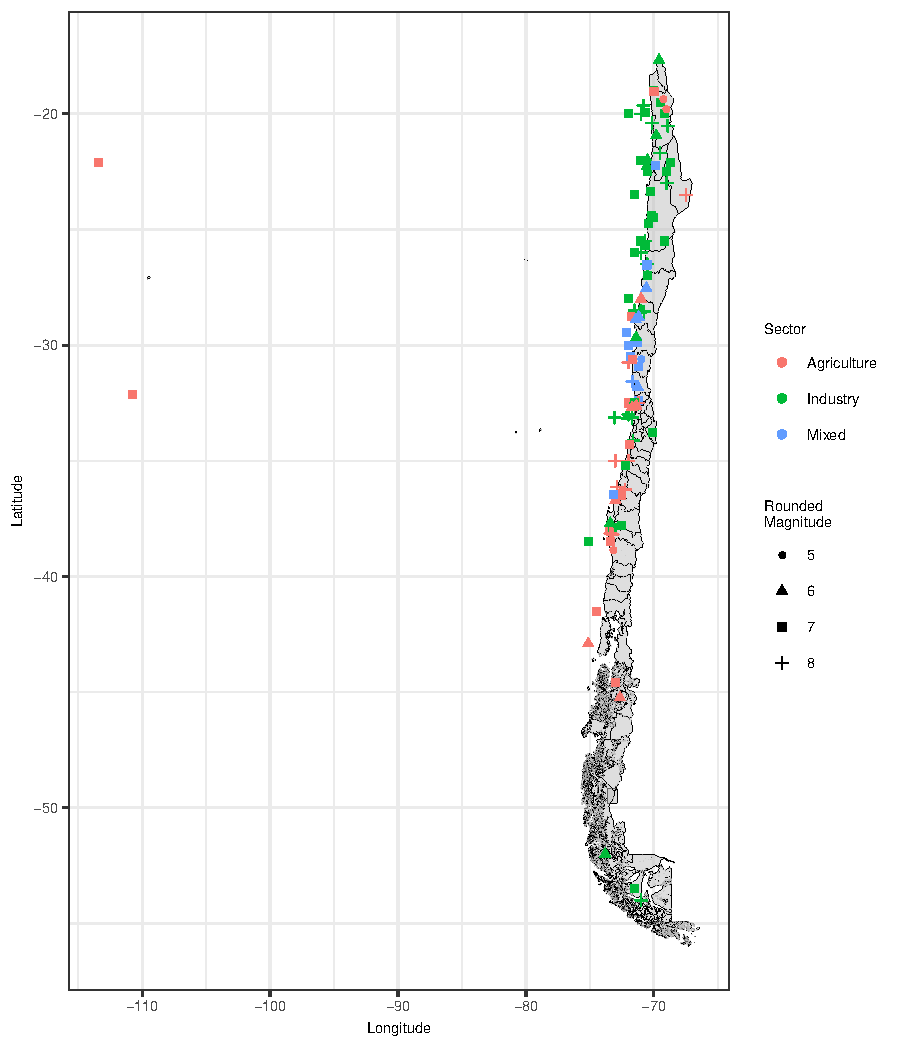
\includegraphics[width=0.7\linewidth]{/Users/hectorbahamonde/RU/Dissertation/Papers/Earthquake_Paper/figure/earthquake:map:plot:chile-1}
\end{minipage}


}


%%%%%%%%%%%%%%%%%%%%%%%%%%%%%%%%%%%%%%%%%%%%%%%%%%%%%%%%%%%%%%%%%%%%%%%%%%%%%%
\headerbox{{\small {\color{textouoh}Income Taxation in Latin America}}}{name=sectionD,column=0,above=bottom}{
%%%%%%%%%%%%%%%%%%%%%%%%%%%%%%%%%%%%%%%%%%%%%%%%%%%%%%%%%%%%%%%%%%%%%%%%%%%%%%
\hspace{1cm}
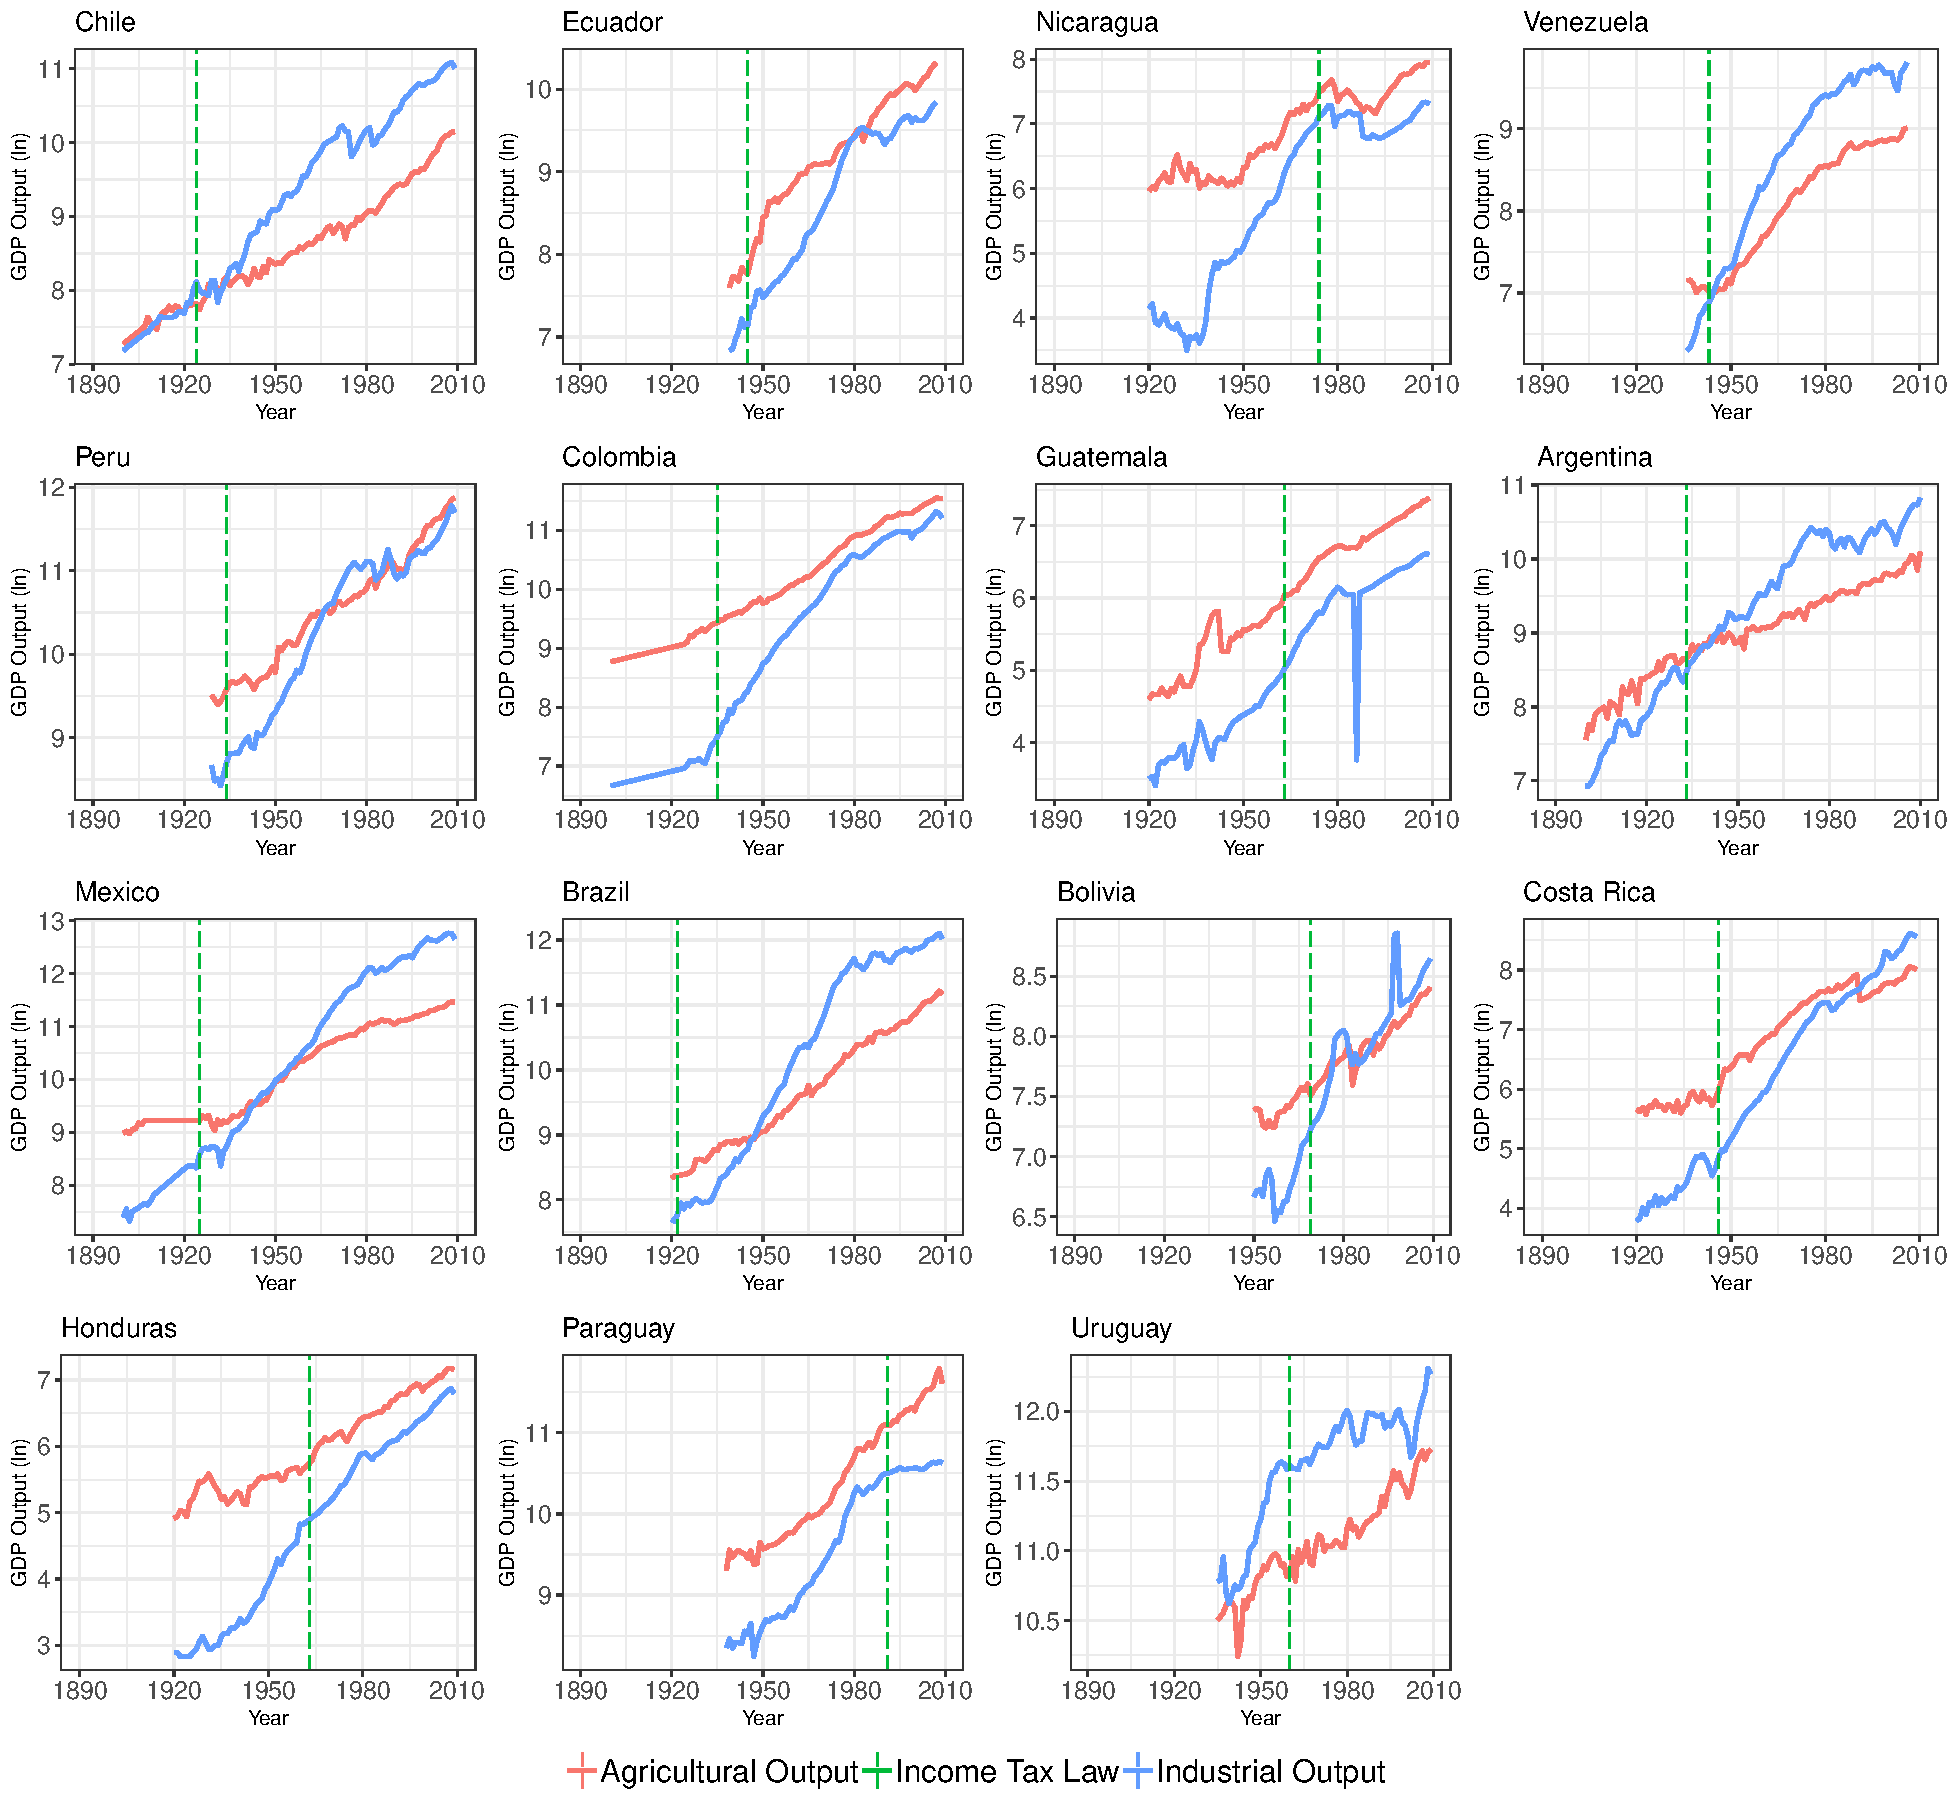
\includegraphics[width=0.65\linewidth]{/Users/hectorbahamonde/RU/Dissertation/Papers/Earthquake_Paper/figure/incometax-1}   
}

%%%%%%%%%%%%%%%%%%%%%%%%%%%%%%%%%%%%%%%%%%%%%%%%%%%%%%%%%%%%%%%%%%%%%%%%%%%%%%
\headerbox{{\color{textouoh}Argument}}{name=sectionE,column=0,above=sectionD,below=sectionB}{
%%%%%%%%%%%%%%%%%%%%%%%%%%%%%%%%%%%%%%%%%%%%%%%%%%%%%%%%%%%%%%%%%%%%%%%%%%%%%%
\vspace{-2mm}\hspace{0.9mm}
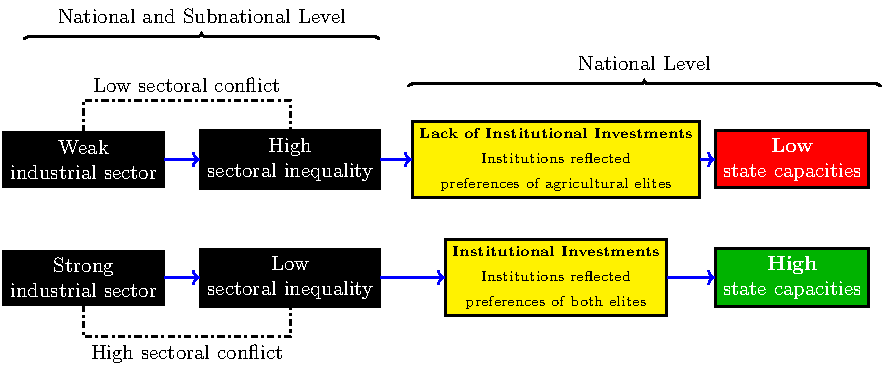
\includegraphics[width=0.85\linewidth]{/Users/hectorbahamonde/RU/Dissertation/Papers/Earthquake_Paper/causal_path}%
}

%%%%%%%%%%%%%%%%%%%%%%%%%%%%%%%%%%%%%%%%%%%%%%%%%%%%%%%%%%%%%%%%%%%%%%%%%%%%%%

\headerbox{{\color{textouoh}Accelerating the Implementation of the Income Tax}}{name=sectionF,column=2,span=2,below=sectionC,above=bottom}{
%%%%%%%%%%%%%%%%%%%%%%%%%%%%%%%%%%%%%%%%%%%%%%%%%%%%%%%%%%%%%%%%%%%%%%%%%%%%%%
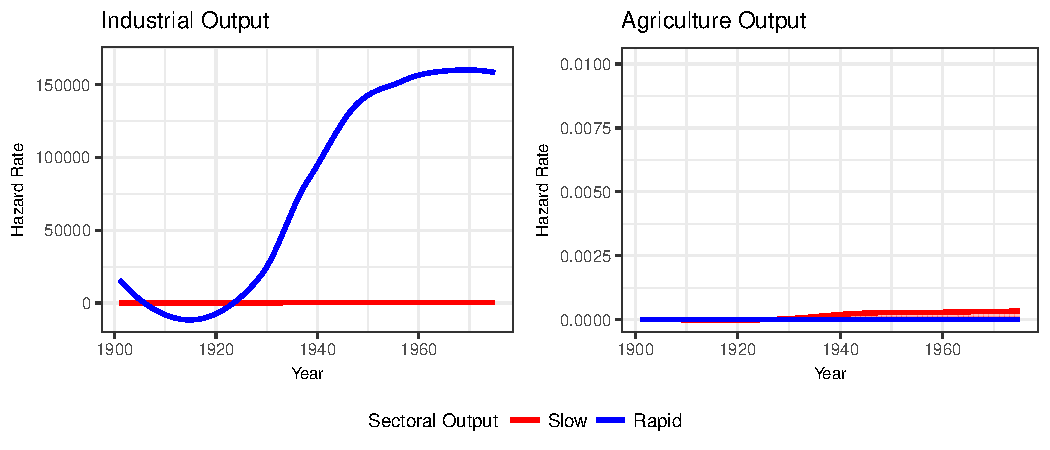
\includegraphics[width=1\linewidth]{/Users/hectorbahamonde/RU/Dissertation/Papers/IncomeTaxAdoption/figure/simulation:plots-1}%

\begin{equation}\label{cox:eq}
h_{i}(t) = exp(\beta_{1}\text{Industrial Growth}_{i,t-1} + \beta_{2}\text{Agricultural Growth}_{i,t-1} + \beta_{3}\text{Total Population}_{i,t-1})h_{0}(t)
\end{equation}
\\
{\bf Simulated Cox Proportional Hazards}. The rise of a strong industrial sector accelerated the implementation of the income tax law in 15 countries in Latin America. Moreover, a strong agricultural sector not only has zero impact on fiscal development, but a negative one.

}
%%%%%%%%%%%%%%%%%%%%%%%%%%%%%%%%%%%%%%%%%%%%%%%%%%%%%%%%%%%%%%%%%%%%%%%%%%%%%%
\headerbox{{\color{textouoh}Earthquake Death Tolls}}{name=sectionG,column=1,span=1,below=sectionC,above=bottom}{
%%%%%%%%%%%%%%%%%%%%%%%%%%%%%%%%%%%%%%%%%%%%%%%%%%%%%%%%%%%%%%%%%%%%%%%%%%%%%%
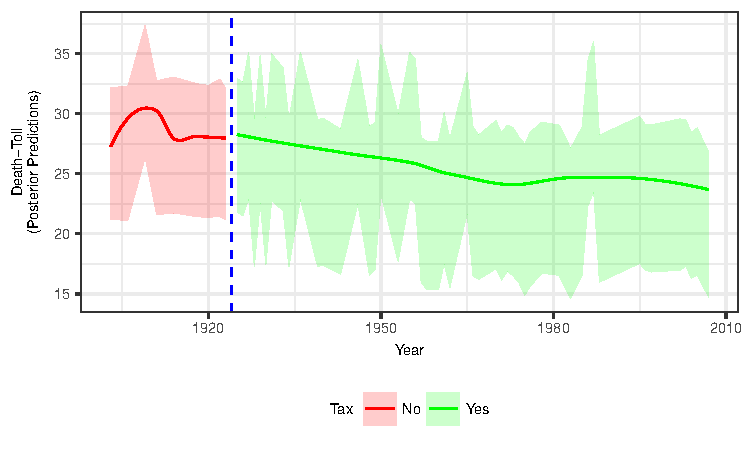
\includegraphics[width=1\linewidth]{/Users/hectorbahamonde/RU/Dissertation/Papers/Earthquake_Paper/figure/income:tax:model:plot:run-1}%

\textbf{Simulated posterior predictions}. The death toll systematically \emph{decreases} over time---i.e. levels of state capacity systematically increase over time---\emph{once the income tax law is implemented}. By implementing the income tax, the baseline propensity of an earthquake increasing the death toll decreases from an estimated over time average of 18 to an estimated over time average of 5.
\\
\\
Both distributions were computed via a {\bf MCMC routine}, particularly the iteration of five chains with 300,000 iterations per chain. Considering the Monte Carlo Markov Chain properties, the first 30,000 observations of every chain were discarded.
}

%%%%%%%%%%%%%%%%%%%%%%%%%%%%%%%%%%%%%%%%%%%%%%%%%%%%%%%%%%%%%%%%%%%%%%%%%%%%%%%
\headerbox{{\color{textouoh}Main Model: Poisson}}{name=algorithm,column=1,above=sectionG,below=sectionA}{
%%%%%%%%%%%%%%%%%%%%%%%%%%%%%%%%%%%%%%%%%%%%%%%%%%%%%%%%%%%%%%%%%%%%%%%%%%%%%%%
\vspace{-1.25em}
{\input{/Users/hectorbahamonde/RU/Dissertation/Papers/Earthquake_Paper/model_poisson.txt}}

The unit of analysis is the earthquake. Each earthquake is associated with a death toll, a location, a magnitude, a local population, and an urban/rural setting. A count model was used to test the effect of implementing the income tax law on earthquake death tolls over time.


}
\end{poster}%
%
\end{document}
